\section{Control Scheme}
Seeing the game is developed for mobile platforms, the main issue is that the main input device is also the screen you are looking at. 
This inheritly requires the control scheme to be designed to obscure the least amount of screen available, as the mobile devices are already rather small. 
Further the screen on a mobile device gives no feedback to the hands which also has to be taken into account.
These two constraints can be formalised as:
\begin{itemize}
\item Minimize the space the input interface requires as much as possible, and make the interface intuitive such that it does not draw attention away from the game.
\item Make sure the input interface is simple to use, such that the need for feedback is minimized as much as possible.
\end{itemize}

\subsection{Similar games control scheme}
In order to make the best possible mobile control scheme, it is relevant to briefly look at some other popular games choices.
Most games seems to use the same \emph{blueprint} in order to make an easy to use interface. Some sort of virtual joypad one the left side of the screen for movement, and then a mix of buttons and joypads on the right side of the screen for actions. 
One of the most popular and well designed games in this category is BombSquad.

\subsection*{BombSquad}
Bombsquad\ref{bombsquad} is a 2.5D action multiplayer game, where the player controls a character whoms goal is to eleminate the opposing characters whom are either player or computer controlled.
The character can move in all directions and it has 4 main abilities. 
The movement input is based on a virtual joystick in the lower left corner.
When the player places the thumb on the joystick, it will work similarily to an ordinary joystick and move the character in the direction the stick is pointing. 
The distance from the thumb/stick to the center of the virtual joystick defines the speed by which the character moves. 
The stick is activated by any finger on the left half of the screen, such that it is not required to actually hit the thumbstick directly with your finger to trigger the input.

The abilities are used in much the same way. 
There are 4 abilities, which can be selected by a mix of touch and thumbstick behaviour. 
Each ability can be activated once by dragging the virtual thumbstick across the designated area for the ability. 
Some abilities, like the sprint, will remain activated as long as a finger is hold upon the ability. 
Other abilities, like the punch, will only trigger once, and require taps on the ability to trigger it again. 
The ability is triggered if any part of ''its'' quarter of the screen is tapped.

\begin{figure}[h]
\centering
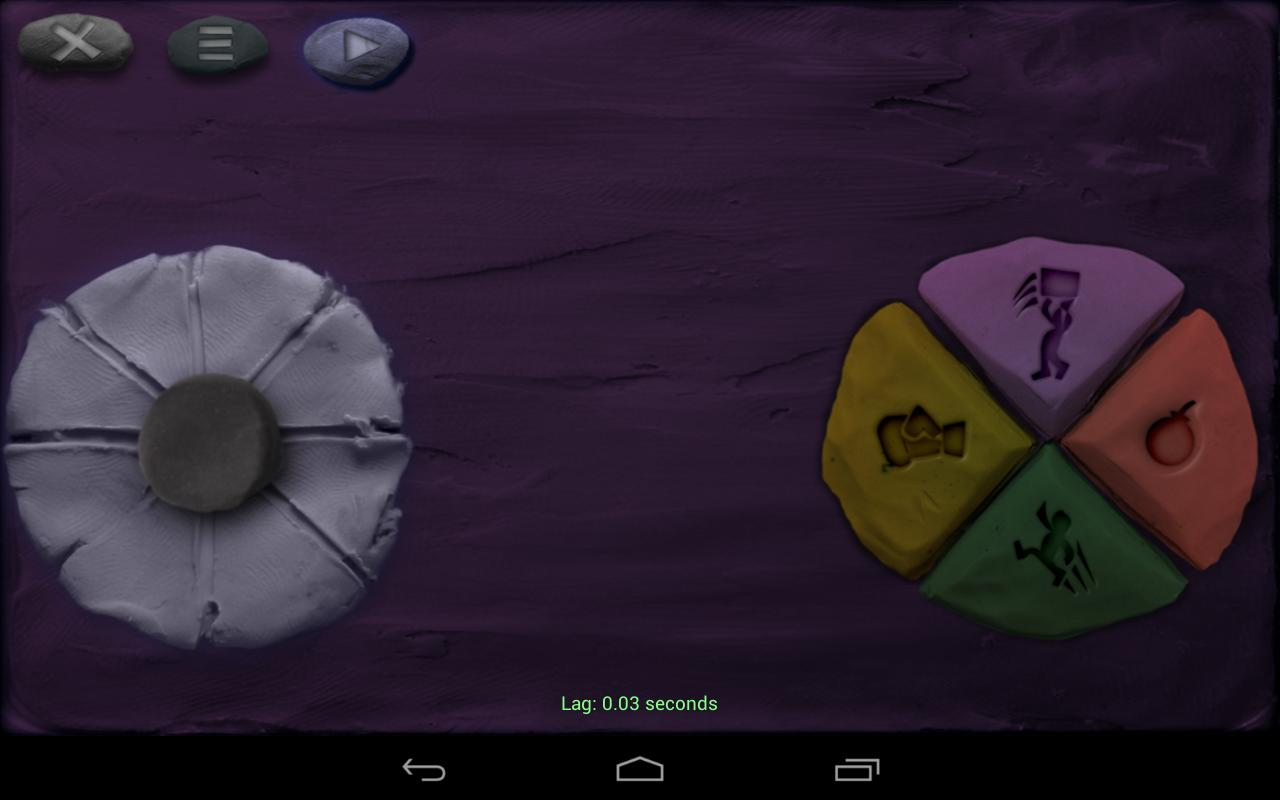
\includegraphics[width=1\textwidth]{figures/analysis/controlscheme/onscreen_control}
\caption{Bombsquad game screen, \url{http://www.froemling.net/wp-content/uploads/2014/04/IMG_1088.jpg}}
\end{figure}

The great thing about this control scheme is that it is compact, easy to use, and allows for focus on the gameplay it self, rather than making sure you are bashing the right buttons when you want to.

Further the game allows usage of controllers if possible. 
This can be done by either connecting a controller to your device (most devices and platforms are supported), and either using your own screen or connecting to a global screen to play at.
This is pretty great, because all the sudden each player can use their own mobile device as an input, and then have a tablet or pc screen as the actual game-screen, removing the conflict of having input and game screen on the same screen.

\begin{figure}[h!]
\centering
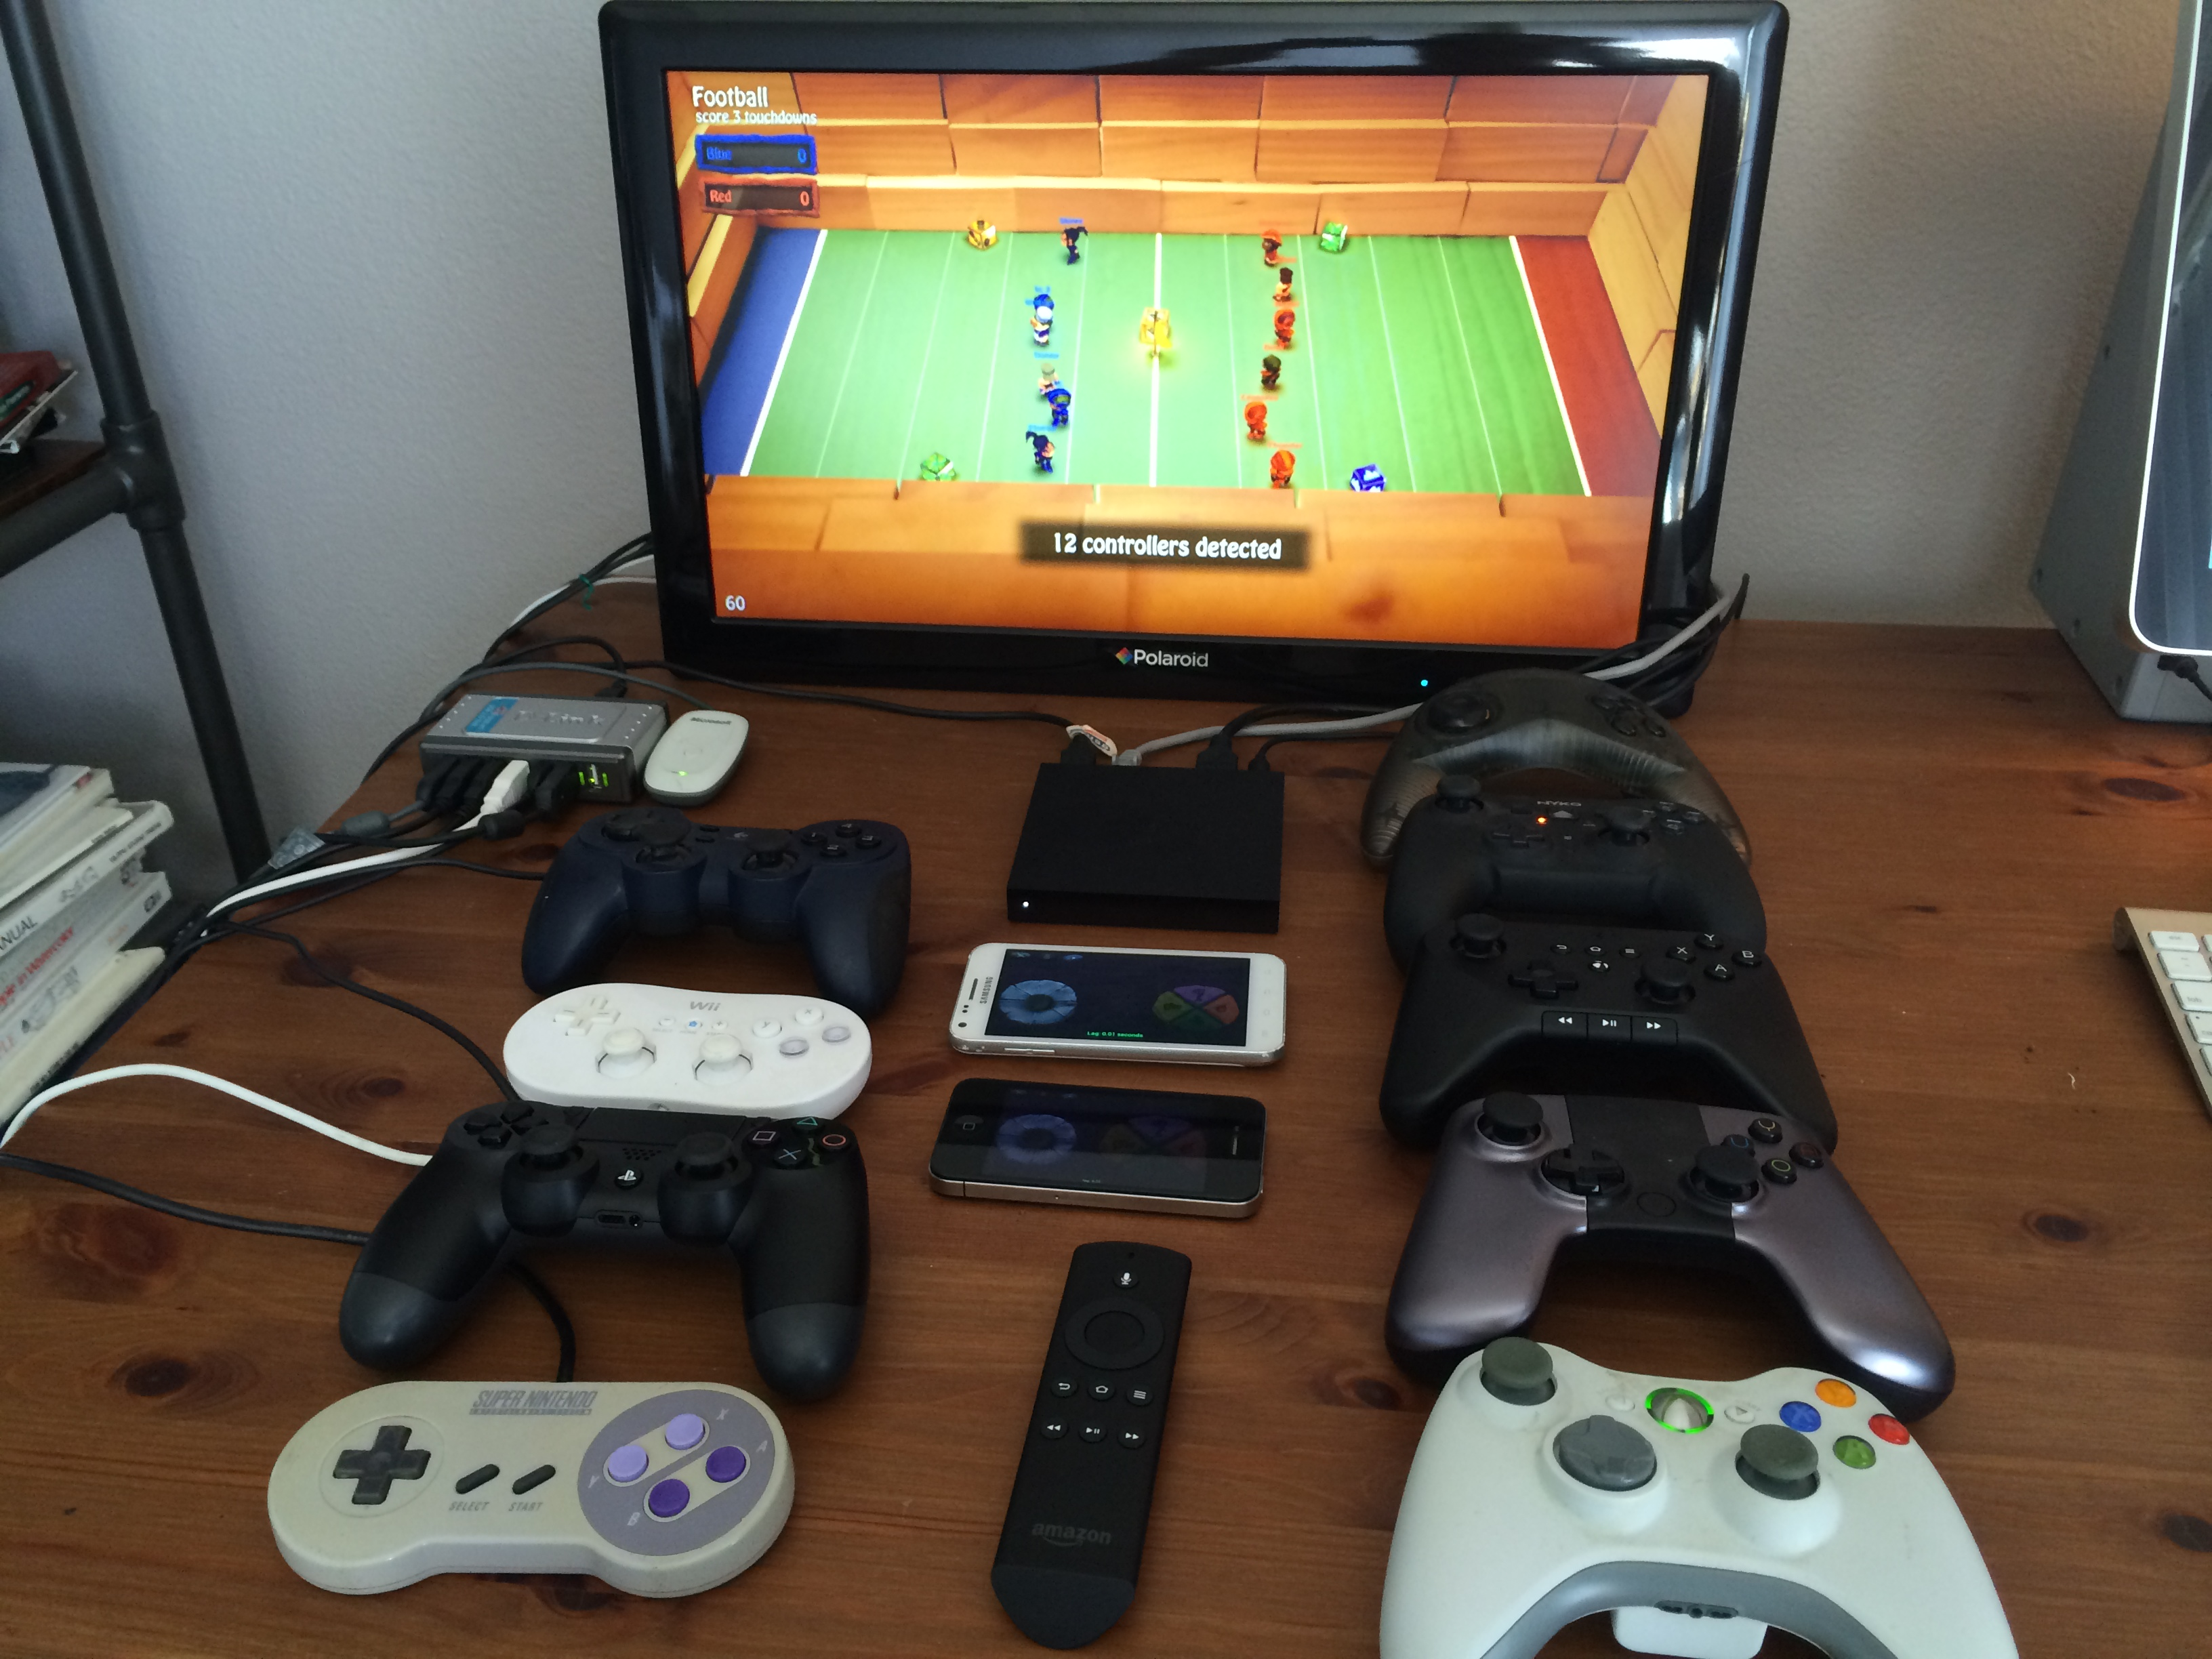
\includegraphics[width=1\textwidth]{figures/analysis/controlscheme/controller_support}
\caption{Bombsquad controller support including a wide range of console controllers and mobile devices, \url{http://www.froemling.net/wp-content/uploads/2014/04/IMG_1088.jpg}}
\end{figure}

\subsection*{Heroes of the Order and Chaos}
Heroes of the Order and Chaos has the same movement scheme as BombSquad. 
Where it differs from BombSquad is in the actions-interface.
It is placed in the right side of the screen as in BombSquad, however, there are quite a few more actions than the four which BombSquad uses.
It includes 4 useable abilities along the right side of the screen, two useable abilities along the bottom of the screen, an \emph{attack} button and a \emph{change target} button.
\begin{figure}[h]
\centering
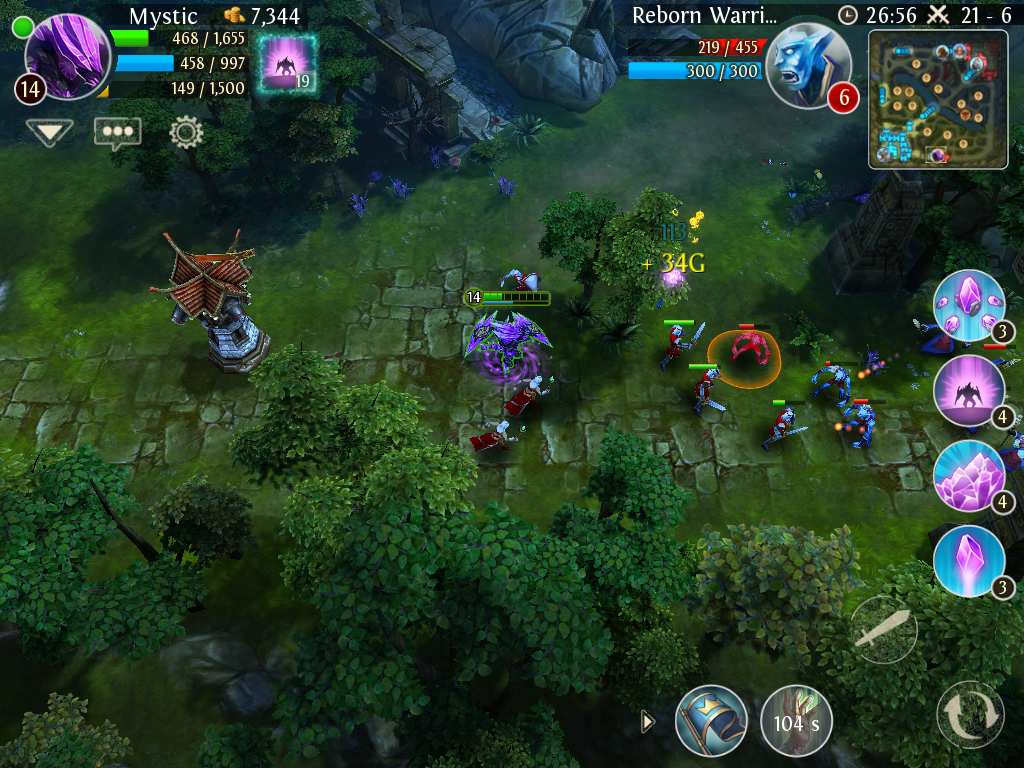
\includegraphics[width=1\textwidth]{figures/analysis/controlscheme/hotoac_control}
\caption{Heroes of the Order and Chaos control interface \url{http://3.bp.blogspot.com/-EQUyarxR56U/ULdIChk_LhI/AAAAAAAAArs/73MwPMoDhnI/s1600/IMG_3227.PNG}}
\end{figure}

The placement of the action buttons make it such that you don't accidently hit the wrong buttons. 
There are quite a few input buttons though, so it takes a bit more getting used to, than the BombSquad interface. 
The buttons are also grouped such that the buttons you usually press in the same situations are at the same place. 
Further some in-game logic has been added such that some of the buttons wont always require pressing (such as attack), and some will queeuee if pressed in succession without the first action being finished.